% Aqui começa o capítulo de Introdução.
% Use o comando \label para definir um rótulo, 
% caso seja necessário referenciar esse capítulo
% posteriormente.
\chapter{Introdução}\label{chp:Introducao}

% TODO: Expandir com contextualização sobre processamento hiperespectral
% Contextualização do problema
O processamento de imagens hiperespectrais representa um desafio computacional significativo devido ao volume massivo de dados e à complexidade dos algoritmos envolvidos. Cada pixel de uma imagem hiperespectral contém informações espectrais de centenas de bandas, resultando em datasets que podem exceder gigabytes de dados \cite{referencia_contextual}.

% TODO: Adicionar estatísticas sobre crescimento de dados hiperespectrais
% TODO: Citar aplicações práticas (agricultura, mineração, medicina, etc.)

\section{Motivação}\label{sec:motivacao}

% TODO: Expandir com justificativas técnicas e econômicas
A escolha entre plataformas de processamento (FPGA vs GPU) para aplicações hiperespectrais é crucial, pois impacta diretamente:
\begin{itemize}
    \item Tempo de processamento em aplicações de tempo real
    \item Consumo energético em sistemas embarcados
    \item Custo de implementação e manutenção
    \item Precisão dos resultados obtidos
\end{itemize}

% TODO: Adicionar dados quantitativos sobre diferenças de desempenho
% TODO: Citar lacunas na literatura sobre comparações sistemáticas

\section{Objetivos}\label{sec:objetivos}

\subsection{Objetivo Geral}
Realizar uma análise comparativa sistemática entre implementações FPGA e GPU para processamento de imagens hiperespectrais, quantificando trade-offs de desempenho, consumo energético e precisão.

\subsection{Objetivos Específicos}
\begin{enumerate}
    \item Implementar algoritmos de pré-processamento hiperespectral em VHDL para simulação FPGA
    \item Desenvolver implementações otimizadas em CUDA para GPU
    \item Estabelecer métricas de comparação objetivas e reproduzíveis
    \item Quantificar diferenças de desempenho entre as plataformas
    \item Identificar cenários ótimos para cada arquitetura
    \item Fornecer diretrizes para seleção de plataforma
\end{enumerate}

% TODO: Refinar objetivos específicos conforme evolução do projeto

\section{Contribuições Esperadas}\label{sec:contribuicoes}

% TODO: Expandir com detalhes sobre originalidade e impacto
Este trabalho contribui para o estado da arte através de:
\begin{itemize}
    \item Primeira comparação sistemática FPGA vs GPU para processamento hiperespectral completo
    \item Implementações otimizadas e reproduzíveis em ambas as plataformas
    \item Metodologia de avaliação padronizada para estudos futuros
    \item Diretrizes práticas para seleção de arquitetura
\end{itemize}

\section{Organização do Texto}\label{sec:organizacao}

% TODO: Ajustar conforme estrutura final dos capítulos
Esta dissertação está organizada da seguinte forma:

\begin{itemize}
    \item \textbf{\Capitulo{chp:levantamento}}: Apresenta o levantamento bibliográfico sobre processamento hiperespectral, arquiteturas FPGA e GPU, e trabalhos relacionados.
    
    \item \textbf{\Capitulo{chp:metodologia}}: Detalha a metodologia experimental, algoritmos implementados, métricas de avaliação e configuração dos experimentos.
    
    \item \textbf{\Capitulo{chp:resultados}}: Apresenta os resultados experimentais obtidos em ambas as plataformas.
    
    \item \textbf{\Capitulo{chp:discussao}}: Analisa e discute os resultados, identificando trade-offs e cenários ótimos.
    
    \item \textbf{\Capitulo{chp:conclusoes}}: Sumariza as conclusões, contribuições e trabalhos futuros.
\end{itemize}

% TODO: Adicionar seção sobre limitações do escopo, se necessário
% TODO: Incluir cronograma de execução na introdução ou metodologia

A seguir, estão alguns exemplos para os elementos mais comuns em textos acadêmicos, \ie tabelas, equações e figuras. 

\section{Exemplos de Tabelas e Equações}\label{sec:exemplostabelas}
Aqui um exemplo de como referenciar a \Tabela{tab:tabela_1}. Note que é preciso definir um rótulo (\textit{label}) dentro do comando de definição da tabela.

% Veja a seguir um exemplo de Tabela.
% Você pode usar o site http://www.tablesgenerator.com
% para gerar as tabelas em LaTeX.
\begin{table}[!htp]
\caption[Legenda curta da tabela]{Legenda longa e mais detalhada da tabela.}
\label{tab:tabela_1}
\begin{center}
\begin{tabular}{cc}
\toprule % Linha superior
Coluna 1 & Coluna2 \\ \midrule % Linha do meio 
a & b \\
c & d \\
e & f \\\bottomrule % Linha inferior
\end{tabular}
\end{center}
\end{table}

As tabelas mais complexas podem ser feitas com ajuda no site \href{http://www.tablesgenerator.com}{http://www.tables\-ge\-ne\-ra\-tor.com}.

Veja um exemplo de equação no próprio texto, \eg, $x=\frac{\sqrt{a^{2}+b^{2}}}{\sigma}$.  Se você preferir, pode escrever a equação de forma estendida, conforme a \Equacao{eq:teste} a seguir. Note que o rótulo é colocado automaticamente.

\begin{equation}
x=\frac{\sqrt{a^{2}+b^{2}}}{\sigma}
\label{eq:teste}
\end{equation}


Você também pode obter ajudar para escrever as equações em \LaTeX no site \url{http://www.codecogs.com/latex/eqneditor.php}.

% Note que podemos incluir automaticamente alguns termos na lista de abreviaturas e siglas no pré-texto. Veja exemplos a seguir no código fonte. 

% A sigla \Sigla{abêcê}{ABC} aparecerá automaticamente na lista de abreviaturas e siglas no pré-texto. Do mesmo modo, podemos usar o comando \SiglaHifen{xisipsilonzê}{XYZ} separado por hífen ao invés de aparecer entre parênteses.

Veja na \Secao{sec:exemplo_secao} a seguir como referenciar uma seção. Também será preciso definir um rótulo (\textit{label}) logo após o comando \texttt{\textbackslash section}.

% Aqui começa uma Seção.
% Use o comando \label para definir um rótulo, 
% caso seja necessário referenciar essa seção
% posteriormente.
\section{Exemplo de seção}\label{sec:exemplo_secao} 
Agora observe como se faz uma citação de artigo científico em periódico \cite{Gradvohl2014c}. De acordo com \textcite{Gradvohl2016}, essa é uma citação direta. Se for citar mais de um trabalho, faça da seguinte forma \cite{Caldana2017,Gradvohl2015}. As referências bibliográficas estão no arquivo \texttt{bibliografia.bib}. Outros exemplos de citações também se encontram nesse arquivo.

Veja a seguir o comando para criar uma figura e o resultado, na \Figura{fig:xwing}. Note, no código fonte, que no comando \texttt{caption} podemos estabelecer uma \enquote{legenda curta} para aparecer na Lista de Figuras. A legenda curta é opcional.

\begin{figure}[!htb]
\centering
% As figuras estão na pasta figuras.
% Se seu texto estiver demorando muito para compilar, use figuras no formato PDF ou PNG.
% Observe, no comando includegraphics que você pode estabelecer uma proporção para a figura.
% Nesse caso, a figura tem uma proporção equivalente à metade (0.5) da largura do texto (\textwidth)
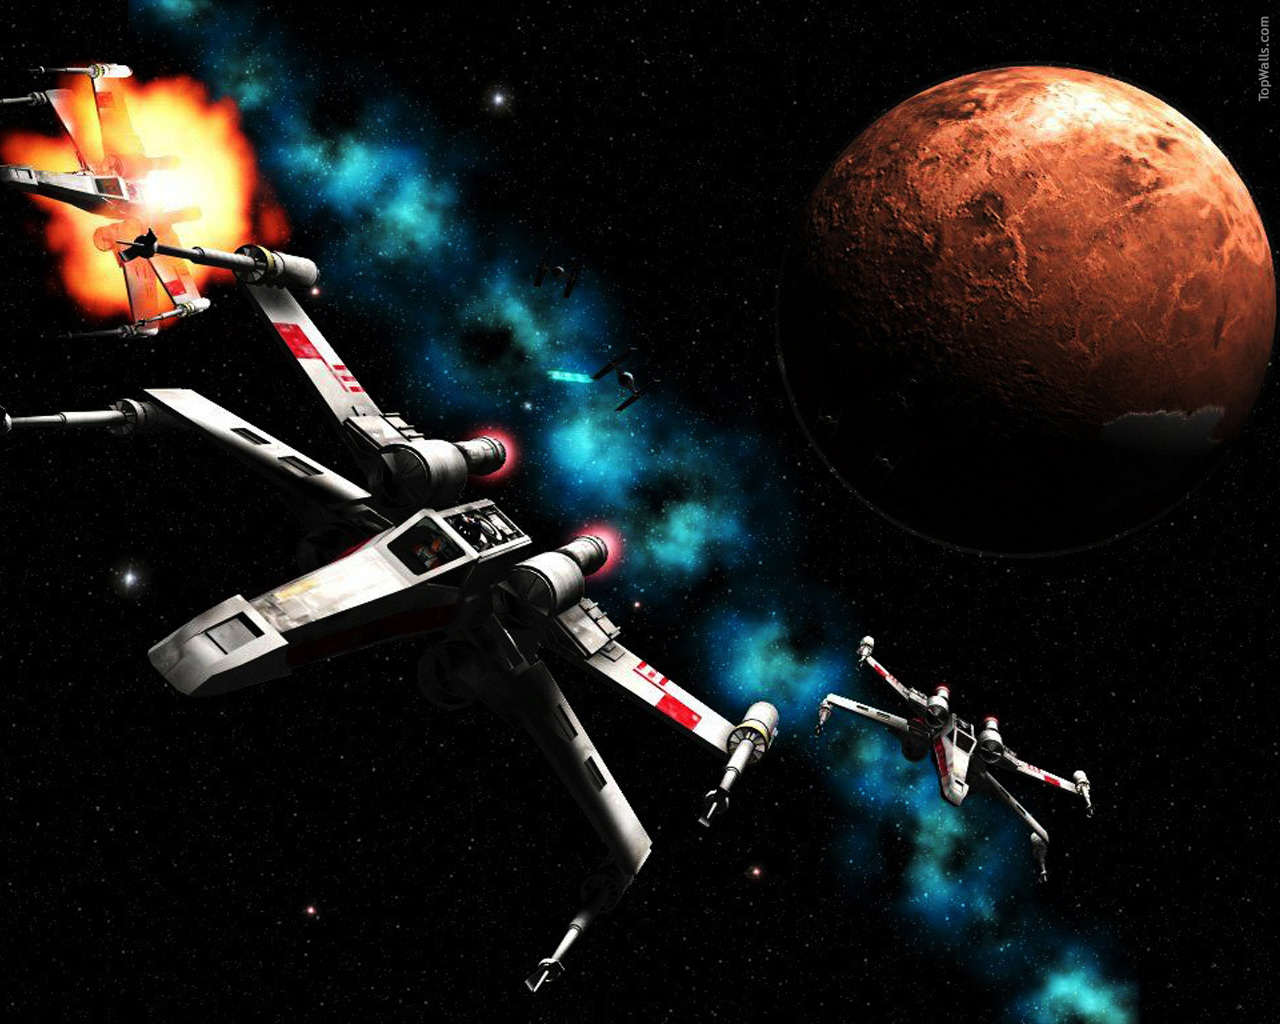
\includegraphics[width=0.5\textwidth]{starwars21280.jpg}
\caption[Legenda curta de figura]{Legenda mais extensa de figura.}
\label{fig:xwing}
\end{figure}

Dica importante: sempre que possível, use figuras no formato PDF. De acordo com o Overleaf, isso acelera a compilação do texto, sem perder a qualidade da figura. 

\subsection{Exemplo de subseção}\label{subsec:exemploSubsec}
É importante evitar chegar a esse nível de subseção. Dois níveis são suficientes. Use essa opção em último caso, apenas.


\subsection{Exemplo de adição de siglas}\label{subsec:siglas}
Para adicionar uma sigla ou abreviatura na lista de siglas e abreviaturas, use o comando ``\texttt{\textbackslash{}Sigla\{nome por extenso\}\{abreviatura\}}'' ou ``\texttt{\textbackslash{}SiglaHifen\{nome por} \texttt{ex\-ten\-so\}\{abreviatura\}}'' para adicionar a sigla com hífen. 
Por exemplo, respectivamente, \Sigla{Ácido Desoxirribonucleico}{DNA} ou \SiglaHifen{Ácido Ribonucleico}{RNA}. A lista de siglas é adicionada automaticamente.

\section{Comandos opcionais para facilitar}\label{sec:comandosOpc}
Este modelo também criou alguns comandos adicionais não apenas para facilitar o trabalho de quem escreve, mas também para manter uma formatação mais consistente.

Entre esses comandos estão o \texttt{\textbackslash{}ie} que inclui a abreviatura ``\ie'' no texto (equivalente ao ``isto é''). Usar esse comando vai garantir que a abreviatura não se separe entre linhas e que o espaço entre o `.' e a próxima letra seja fixo. O mesmo vale para os comandos \texttt{\textbackslash{}eg} que inclui a abreviatura ``\eg'' e \texttt{\textbackslash{}pex} que inclui a abreviatura ``\pex''.

Também existem os comandos \texttt{\textbackslash{}Capitulo\{rótulo do capítulo\}}, \texttt{\textbackslash{}Equacao\{ró\-tu\-lo da equação\}}, \texttt{\textbackslash{}Figura\{rótulo da figura\}}, \texttt{\textbackslash{}Secao\{rótulo da seção\}} e \texttt{\textbackslash{}Tabela\{rótulo da tabela\}}. Esses comandos inserem referências para os respectivos elementos. Além disso, no próprio texto aparece a \textit{string} (``Capítulo'', ``Equação'', ``Figura'' etc) seguida da referência já com o link. Por exemplo, \Secao{sec:exemplo_secao}. Sugere-se a utilização desses comandos para referenciar os respectivos elementos ao invés do comando \texttt{\textbackslash{}ref\{rótulo\}}. Assim, o texto ficará mais uniforme. 

É possível também usar esses comandos nas versões no plural para conjuntos de referências. Por exemplo, para referenciar várias seções, você pode utilizar o comando \texttt{\textbackslash{}secoes\{ró\-tu\-lo\_1, rótulo\_2, rótulo\_3\}}.

Por exemplo, suponha que queiramos referenciar as \secoes{sec:exemplostabelas,sec:exemplo_secao,subsec:siglas}.